\renewcommand*\chappic{img/diff-crypt.pdf}
\renewcommand*\chapquote{Just because it's automatic doesn't mean it works.}
\renewcommand*\chapquotesrc{Daniel J. Bernstein}
\chapter{Differential cryptanalysis}
\label{ch:dc}
%
\section{MD4}
\label{sec:dc-md4}
%
\index{MD4}
MD4 is a cryptographic hash function originally described in RFC~1186~\cite{rfc1186},
updated in RFC~1320~\cite{rfc1320} and declared obsolete by RFC~6150~\cite{rfc6150}. It was
invented by Ronald Rivest in 1990 with properties given in Table~\ref{tab:md4}.
Since 1995~\cite{Dobbertin1998} successful attacks have been found to break collisions,
preimage and second-preimage resistance in MD4; including but not limited to~\cite{md4-2007} and
\cite{cryptoeprint:2005:151}. A Python~3 implementation derived from a previous Python version
is available at github~\cite{md4-py3k}.

\begin{table}[h]
  \begin{center}
    \begin{tabular}{lcl}
      block size           & 512 bits       & namely variable \texttt{block} in RFC~1320~\cite{rfc1320} \\
      digest size          & 128 bits       & as per Section~3.5 in RFC~1320~\cite{rfc1320} \\
      internal state size  & 128 bits       & namely variables $A$, $B$, $C$ and $D$ \\
      word size            & 32 bits        & as per Section~2 in RFC~1320~\cite{rfc1320} \\
    \end{tabular}
    \caption{MD4 hash algorithm properties}
    \label{tab:md4}
  \end{center}
\end{table}

MD4 uses three auxiliary Boolean functions:
\begin{align}
  \IF(X,Y,Z) &= (X \land Y) \lor (\neg X \land Z) \\
  \MAJ(X,Y,Z) &= (X \land Y) \lor (X \land Z) \lor (Y \land Z) \\
  \XOR(X,Y,Z) &= (X \land \neg Y \land \neg Z) \lor (\neg X \land Y \land \neg Z) \nonumber\\
              &\lor (\neg X \land \neg Y \land Z) \lor (X \land Y \land Z)
\end{align}

\begin{defi}
  The Boolean \boolf{IF} function behaves the following way:
  If the first argument is true, the second argument is returned.
  If the first argument is false, the third argument is returned.

  The Boolean \boolf{MAJ} function returns true if the number
  of Boolean values true in arguments is at least $2$.
  The Boolean \boolf{XOR} function returns true if the number
  of Boolean values true in arguments is odd.
\end{defi}

In the following a quick overview over MD4's design is given.

\begin{description}
  \item[Padding and length extension]
    First of all, padding is applied. A single bit 1 is appended to the
    input. As long as the input does not reach a length congruent 448 modulo 512,
    bit 0 is appended.
    Followingly, length appending takes place. Represent the length of the input
    (without the previous modifications) in binary and take its first
    64 less significant bits. Append those 64 bits to the input.
  \item[Initialization]
    The message is split into 512-bit blocks (i.e. 16 32-bit words).
    Four state variables $A$, $B$, $C$ and $D$ are initialized with these
    hexadecimal values:
    \[
      \mathtt{[A]}\; \texttt{01234567} \quad
      \mathtt{[B]}\; \texttt{89abcdef} \quad
      \mathtt{[C]}\; \texttt{fedcba98} \quad
      \mathtt{[D]}\; \texttt{76543210}
    \]
  \item[Round function with state variable updates]
    We also need an auxiliary matrix $(i_{k,l})$ which stores indices.
    Let $i_{k,l}$ be the value in the $k$-th row and $l$-th column of matrix $(i_{k,l})$.
    Analogously $j_{k,l}$ is defined for matrix $(j_{k,l})$.
    %
    \[
      (i_{k,l}) = \left(\begin{array}{cccccccccccccccc}
        0 & 1 & 2 & 3 & 4 & 5 & 6 & 7 & 8 & 9 & 10 & 11 & 12 & 13 & 14 & 15 \\
        0 & 4 & 8 & 12 & 1 & 5 & 9 & 13 & 2 & 6 & 10 & 14 & 3 & 7 & 11 & 15 \\
        0 & 8 & 4 & 12 & 2 & 10 & 6 & 14 & 1 & 9 & 5 & 13 & 3 & 11 & 7 & 15
      \end{array}\right)
    \] \[
      (j_{k,l}) = \begin{pmatrix}
        3 & 7 & 9 & 11 \\
        3 & 5 & 9 & 13 \\
        3 & 9 & 11 & 15
      \end{pmatrix}
    \]
    %
    Then the round function is applied to this block in three rounds
    with 16 iterations each. Let $1 \leq k \leq 3$ be the round counter
    and $1 \leq l \leq 16$ be the iteration counter. For every round,
    for every iteration apply the following function:

    The values of state variable $B$, $C$ and $D$ are taken as arguments
    for function $F$ where $F$ is \boolf{IF} in the first 16 iterations,
    \boolf{MAJ} in the following 16 iterations and finally \boolf{XOR}
    in the last 16 iterations. This return value is added to the value of state
    variable $A$, the current message block $M_i$ and $X[i_{k,l}]$. This sum is then left-rotated by
    $j_{k,l \bmod{4}}$ bits and stored in value B. State variables $B$, $C$ and
    $D$ update variables $C$, $D$ and $A$ respectively.
    
    This round function design is visualized in Figure~\ref{fig:md4-round-function}.
\end{description}

\begin{figure}[p]
  \begin{center}
    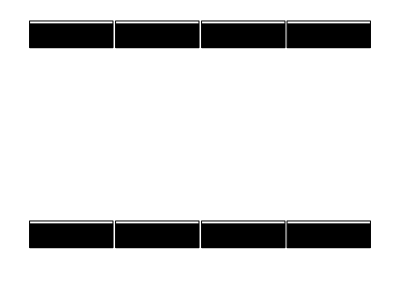
\includegraphics{img/md4.pdf}
    \caption{MD4 round function updating state variables $A$, $B$, $C$ and $D$}
    \label{fig:md4-round-function}
  \end{center}
%\end{figure}
%\begin{figure}[p]
  \begin{center}
    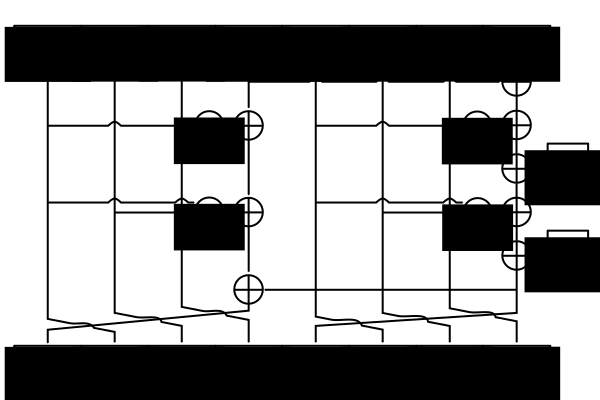
\includegraphics[width=\textwidth]{img/sha256.pdf}
    \caption{SHA-256 round function}
    \label{fig:sha256-round-function}
  \end{center}
\end{figure}

\section{SHA-256}
\label{sec:dc-sha-256}
%
\index{SHA-256}
SHA-256 is a hash function from the SHA-2 family designed by the National Security Agency (NSA)
and published in 2001. It uses a Merkle-Damg\aa{}rd construction with a Davies-Meyer
compression function.
% TODO: reference to standard
% https://web.archive.org/web/20130526224224/http://csrc.nist.gov/groups/STM/cavp/documents/shs/sha256-384-512.pdf

\begin{table}[h]
  \begin{center}
    \begin{tabular}{lcl}
      block size           & 512 bits       & as per Section~2.2 of the standard \\
      digest size          & 256 bits       & as per Section~1 of the standard \\
      internal state size  & 256 bits       & as per Section~2.2 of the standard \\
      word size            & 32 bits        & as per Section~2.2 of the standard \\
    \end{tabular}
    \caption{SHA-256 hash algorithm properties}
    \label{tab:sha256}
  \end{center}
\end{table}

Besides MD4's two auxiliary functions \boolf{MAJ} and \boolf{IF},
another two auxiliary functions are defined:

\begin{align}
  \Sigma_0(X,Y,Z) &= S^2(x) \oplus S^{13}(x) \oplus S^{22}(x) \\
  \Sigma_1(X,Y,Z) &= S^6(x) \oplus S^{11}(x) \oplus S^{25}(x)
\end{align}

\begin{description}
  \item[Padding and length extension]
    The padding and length extension scheme of MD4 is used also in SHA-256.
    Append bit 1 and append single bits 0 until the message reaches a length
    of $448 \mod{512}$. Afterwards the first 64 bits of the binary representation
    of the original input is appended.
  \item[Initialization]
    In a similar manner to MD4,
    initialization of internal state variables takes place before running the
    round function.
    \[
      \begin{array}{llll}
        H_1^{(0)} = \texttt{6a09e667} &
        H_2^{(0)} = \texttt{bb67ae85} &
        H_3^{(0)} = \texttt{3c6ef372} &
        H_4^{(0)} = \texttt{a54ff53a} \\
        H_5^{(0)} = \texttt{510e527f} &
        H_6^{(0)} = \texttt{9b05688c} &
        H_7^{(0)} = \texttt{1f83d9ab} &
        H_8^{(0)} = \texttt{5be0cd19}
      \end{array}
    \]
  \item[Round function]
    For every block of 512 bits, the round function is applied.
    The round function entails a much larger internal state than MD4.


\end{description}

\section{Differential notation}
\label{sec:dc-notation}
%
\cite{char-2006}

\begin{table}[b]
  \begin{center}
    \begin{tabular}{cp{5cm}cl}
      bit condition  & conjunctive normal form &
      bit condition  & conjunctive normal form \\
    \hline
      \dnI{\#}        & $(z) \land (\neg z)$ &
      \dnI{1}         & $(z) \land (z^*)$ \\

      \dnI{0}         & $(\neg z) \land (\neg z^*)$ &
      \dnI{-}         & $\neg (z \oplus z^*)$ \\

      \dnI{u}         & $(z) \land (\neg z^*)$ &
      \dnI{A}         & $(z)$ \\

      \dnI{3}         & $(\neg z^*)$ &
      \dnI{B}         & $(z \lor \neg z^*)$ \\

      \dnI{n}         & $(\neg z) \land (z^*)$ &
      \dnI{C}         & $(z^*)$ \\

      \dnI{5}         & $(\neg z)$ &
      \dnI{D}         & $(\neg z \lor z^*)$ \\

      \dnI{x}         & $(z \oplus z^*)$ &
      \dnI{E}         & $(z \lor z^*)$ \\

      \dnI{7}         & $(\neg z \lor \neg z^*)$ &
      \dnI{?}         &  \\
    \end{tabular}
    \caption[Simple Evaluation clauses]{
        Set bit condition value clauses in Simple Evaluation added for a bit condition.
        A bit condition corresponds to two boolean variables $z$ and $z^*$.
    }
    \label{tab:simple-eval-clauses}
  \end{center}
\end{table}


\section{Addition example}
\section{Differential path}
